\documentclass{scrartcl}

\usepackage[utf8]{inputenc}
\usepackage{amsmath}
\usepackage{amsthm}
\usepackage{amssymb}
\usepackage{geometry}
\usepackage{mathtools}
\usepackage{cancel}
\usepackage{xfrac}
\usepackage{siunitx}                    % for scientific notation \num{}
\usepackage{authblk}                    % for authors
\usepackage{tikz}                       % for circled {}
\usepackage{systeme}                    % for system of equations bracket
\usepackage{verbatim}                   % for comment
\usepackage{xfp}                        % for floating point operations in macros
\usepackage{graphicx}                   % for cropping the images
\usepackage{dsfont}                     % for doublestroke fonts
\usepackage{float}
\usepackage{hyperref}                   % hyperlink
\usepackage[english]{babel}
\usepackage[square, numbers]{natbib}
\usepackage[nottoc]{tocbibind}          % Includes "References" in the table of contents

\bibliographystyle{abbrvnat}

\hypersetup{
	colorlinks=true, 
	citecolor=blue,
}

\AtBeginDocument{\renewcommand{\bibname}{References}}

\title{Video Prediction}
\subtitle{Independent Work Report (MAE 340, Spring 2021)}
\author{Matthew Coleman}
\date{April 26, 2022}

\begin{document}

\maketitle

\vspace{8cm}
\Large
\textit{This project represents my own work, in accordance with the University regulations.} \\
\hspace*{\fill} \large /s/Matthew Coleman
\normalsize

\newpage
\tableofcontents
\newpage

\section{Introduction}
\label{sec:intro}

While humans cannot perfectly predict the future, they are indeed capable of
inferring a great deal of information about near events in the future, and this
knowledge greatly aids them in planning out their actions, such as which
movements to take to reach a goal. This ability to forecast the future is a
direct result of an understanding of causality that is learned through
observation and interaction \cite{human_learning_sequences}.

A great amount of human predictions are, of course, erroneous in major
respects, but even the humans least adept at inferring far-off outcomes and
consequences still are masters of learning very near-term ones. For example,
humans have a good sense for where a car will move in the street, or which
direction a pedestrian may continue walking. Even a young child can predict
where to toss a football to a moving receiver, and even this small knowledge
reveals an infinite wisdom compared to the most advanced video prediction
methods.

The task of video prediction is comprised of several open challenges in
computer vision; it uses some of the most recent model architectures that have
been developed and it even contends directly with an impossible task
altogether, which is to predict the future. Although it is a particularly
confusing task, it also has the potential for immense impact and immediate
practical applications, such as in autonomous driving \cite{eg_self_driving},
video interpolation \cite{eg_video_interp} and most interesting in the context
of this report, robotic control systems \cite{eg_robot_control}.

This project will examine the current state-of-the-art in video prediction
models, report on several experiments carried out by implementing and testing
such a model on various existing datasets, and attempt to make meaningful
conclusions about video prediction and learning causality.

\section{The Task of Video Prediction}
\label{sec:task}

\newcommand{\Xseq}{$\boldsymbol{X} = \left( X_1 , X_2 , X_3 \cdots X_n \right)$}
\newcommand{\Yseq}{$\boldsymbol{Y} = \left( Y_1 , Y_2 , Y_3 \cdots Y_m \right)$}
\newcommand{\Yhatseq}{
	$\hat{\boldsymbol{Y}} = 
	\left( \hat{Y}_1 , \hat{Y}_2 , \hat{Y}_3 \cdots \hat{Y}_n \right)$
}

The task of video prediction is to construct an approximation for the
completion of a sequence of frames, given only the initial sequence of frames.
Formally, given an ordered set of $n$ image frames \Xseq, the task is to
predict the latter $m$ frames of the sequence \Yseq, each frame of which having
the same dimensions, for example with $c$ channels, height $h$, and width $w$.
At each inference in training, the model predictions \Yhatseq, with the same
dimensions as the inputs, are conditioned on the input sequence
$\boldsymbol{X}$, and the model weights are updated typically by the gradient
of a loss function computed between the predictions and ground truth sequence
$\boldsymbol{Y}$ directly. Critically, since there is no human intervention or
labeling required for the model to do this, and models typically are able to
learn from the implicit temporal organiziation of the video data, video
prediction is a self-supervised task \cite{video_prediction_survey}.

% A great deal of discussion in video prediction research centers around exactly
% how these predictions are computed, specifically by testing different model
% architectures, loss functions, and training approaches, however, there is also
% a good amount of disagreement on how model predictions are actually evaluated.
% For example, models trained using pixel-wise loss functions such as MSE will
% typically prefer blurrier predictions in order to capture the underlying
% stochasticity of the data, whereas GANs will prefer to produce more realistic
% data, even if the predictions are further off the mark.

\newpage
\section{Families of Prediction Models}
\label{sec:families}

Modern video prediction models tend to adopt several canonical architectures,
which are normally simple and easily generalizable for specific tasks, such
that they can be used as building blocks or blueprints within larger
architectures. Understanding what each architecture seeks to do on a high level
is imperative to understanding what kind of output one should expect from the
model, since they are each very unique, and research implementations make use
of them in different ways.

For example, RNNs and generative networks are each successful and well-tested
paradigms used in many other machine learning domains outside of computer
vision, but they are especially utilized within video prediction because of
their key properties and strengths, particularly of RNNs to work on
time-sequential data and of generative networks to ``imagine'' new data within
a distribution. These paradigms are used extensively in Convolutional LSTM,
FutureGAN \cite{futuregan}, and SAVP models \cite{savp}, as well as many other
models in cutting-edge research. A short description of each family and its
relevance to video prediction is given below:

\subsection{Recurrent Neural Networks}
\label{subsec:recurrent}

Formally, a Recurrent Neural Network (RNN) is the end-result of a mathematical
analysis of a nonlinear first-order non-homogeneous ordinary differential
equation describing the time-evolution of a state signal $\vec{s}$ as a
function of time, along with an input signal $\vec{x}$. The canonical statement
of an RNN is given below in the form of a discrete Delay Differential Equation
(DDE) \cite{rnn_and_lstm_fundamentals}:

\begin{equation}
	\begin{split}
		\vec{s} [t] & = W_s \vec{s} [t - 1] + W_r \vec{r} [t - 1] + W_x \vec{x} [t] + \vec{\theta_s} \\
		\vec{r} [t] & = G ( \vec{s} [t] )
	\end{split}
	\label{eq:rnn_canonical}
\end{equation}

With $W_s$, $W_r$, and $W_x$ as weight matrices which are either multiplied or
convolved with their respective signals, and $\vec{\theta_s}$ as a bias term
which is typically added in element-wise fashion to $\vec{s}$. This equation
also includes the read-out or output signal $\vec{r}$, which is the activation
$G(z)$ of the state signal, and can be seen as the ``output'' of the network.
All together, this equation describes all of the moving parts of an RNN.

A more understandable depiction of the RNN described in Equation
\ref{eq:rnn_canonical} can be found in Figure \ref{fig:rnn_arch}. This figure
also shows the ``unfolding'' or ``unrolling'' of the model, which is just a way
of seeing each time-step of the state signal $\vec{s} [t]$, input signal
$\vec{x} [t]$, and ouput signal $\vec{r} [t]$ (here replaced by $\hat{y} [t]$,
denoting the network inferences) as they are produced over time.

\begin{figure}[H]
	\begin{center}
		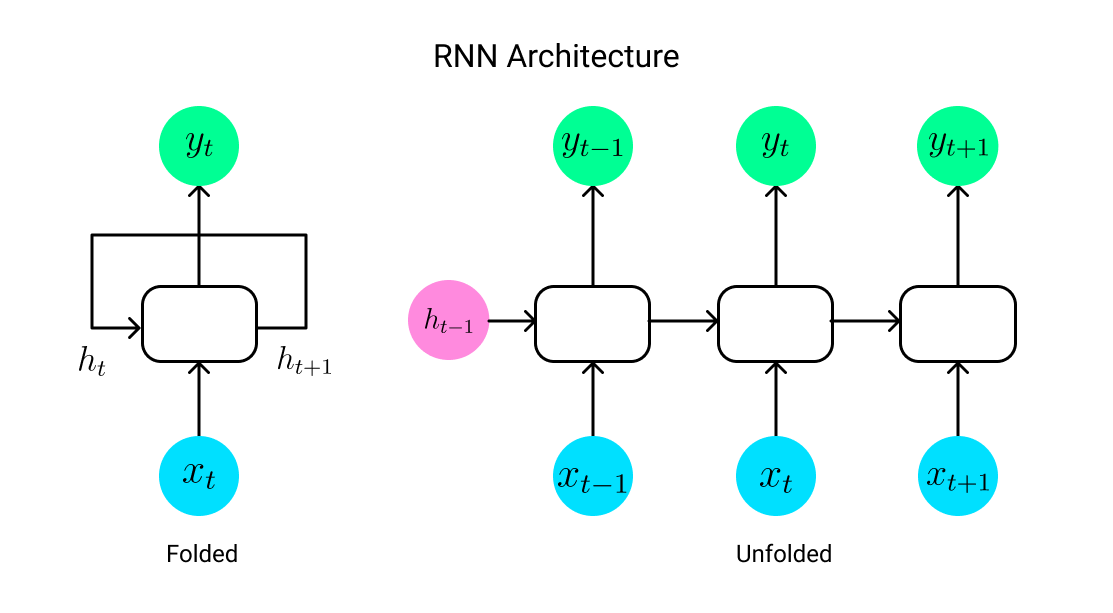
\includegraphics[width=1\textwidth]{figures/rnn_arch.png}
	\end{center}
	\caption{RNN Architecture}
	\label{fig:rnn_arch}
\end{figure}

% Recurrent neural networks (RNNs) consist of a network of nodes that stretches
% over some sequential information, typically in the form of a time sequence
% (Which is the case in video prediction). Each node will perform another
% learning technique on the data in sequence (This could be a convolution
% operation, a linear layer, or a combination of several, for example) and output
% its own activation. Commonly, this is implemented not with a network of
% individual nodes but rather in the form of a feedback loop over a single node,
% which passes some data embedding forward through the network to itself in a
% loop (a hidden state, or variable), only taking in new data from the original
% input sequence at each step. In this way, an RNN equipped with convolution is
% capable of learning from time-varying information while preserving
% spatio-temporal relations (That is, relationships in the data that exist over
% space, such as the shape of a person's leg and hip, as well as relationships in
% the data that exist over time, such as the motion of a person walking, will be
% preserved in the final activations of the network).

% The outputs of each node are then used for other purposes, depending on the
% task, and the result is then backpropagated against a loss function. In machine
% learning terminology, this is referred to as backpropagation through time
% (BPTT) \cite{rnn_and_lstm_fundamentals}, since a gradient must be computed in
% the input sequence's reverse order, i.e., backwards through time, and in the
% case of an RNN implemented with feedback, this gradient must be computed with
% respect to the input data at each time step and then added to the weights of
% the single node in sum.

\subsection{Generative Models}
\label{subsec:generative}

\begin{figure}[H]
	\begin{center}
		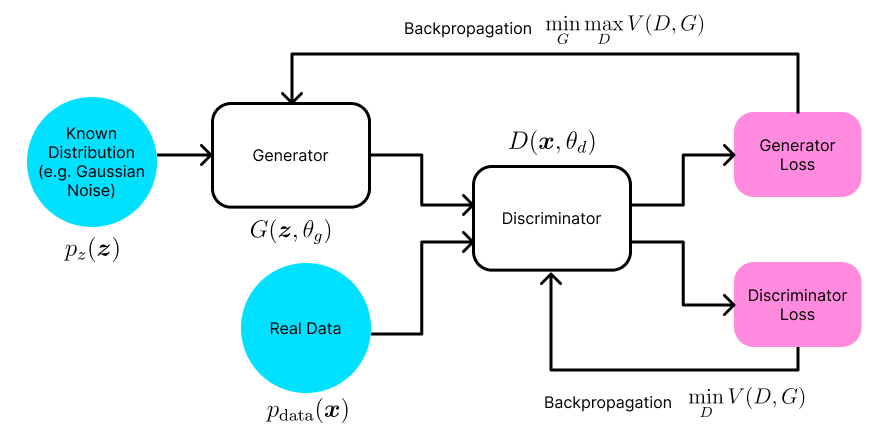
\includegraphics[width=1\textwidth]{figures/gan_arch.png}
	\end{center}
	\caption{General GAN Architecture}
	\label{fig:gan_arch}
\end{figure}

Generative neural networks (for example, GANs) consist of mostly the same
architecture as discriminative neural nets, such as the ones which are
classically used for image classification. While discriminative nets seek to
learn the conditional probability $p(y \mid x)$ of an input $x$ belonging to a
particular class $y$, generative nets seek to learn the conditional probability
distribution $p(x \mid y)$ of an input data given the output, allowing them to
make inferences in the form of ``imagined'' data that might belong to the same
distribution as $x$ \cite{gan_original}. In short, discriminative models would
look at many Van Gogh paintings and fakes in order to learn to differentiate
between them, and generative models would look at many Van Gogh paintings in
order to learn how to paint like Van Gogh.

In practice, this is done by passing a low-dimensional embedding vector from a
known latent distribution (such as the kind that may come as an activation from
a discriminative net) through a typical network in reverse, generating an
upscaled output in the same shape as the targeted learning data.

\section{Video Prediction Models}
\label{sec:families}

\subsection{Convolutional LSTM}
\label{subsec:conv_lstm}

\begin{figure}[H]
	\begin{center}
		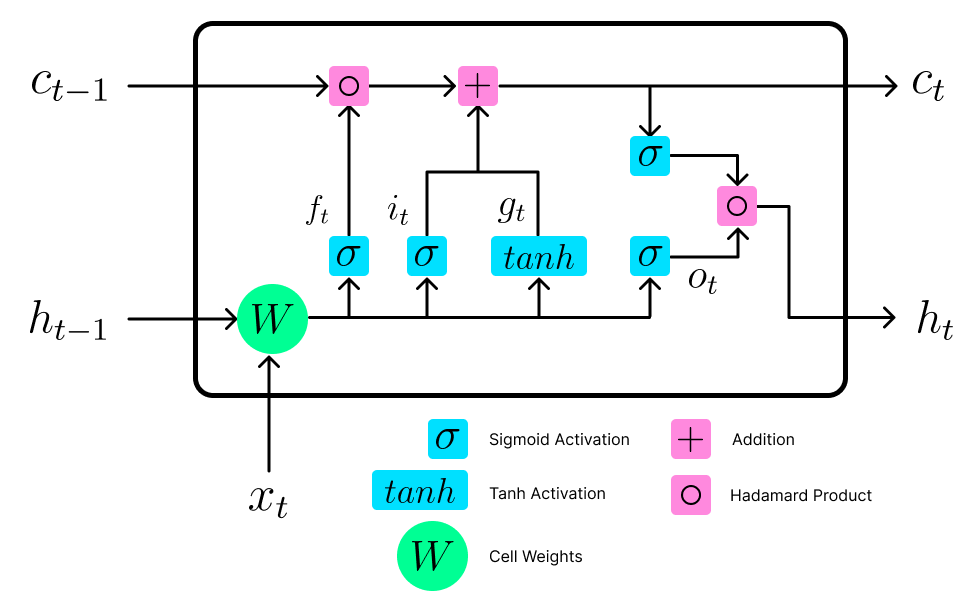
\includegraphics[width=1\textwidth]{figures/lstmcell_arch.png}
	\end{center}
	\caption{LSTM Cell Architecture}
	\label{fig:lstmcell_arch}
\end{figure}

\begin{figure}[H]
	\begin{center}
		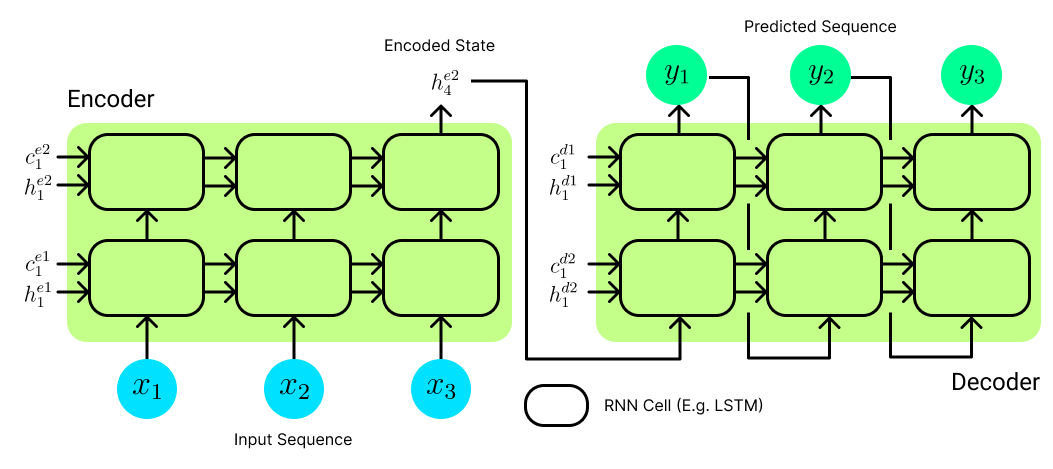
\includegraphics[width=1\textwidth]{figures/seq2seq_arch.png}
	\end{center}
	\caption{Seq2Seq Architecture}
	\label{fig:lstmcell_arch}
\end{figure}


\subsection{FutureGAN}
\label{subsec:futuregan}

\begin{figure}[H]
	\begin{center}
		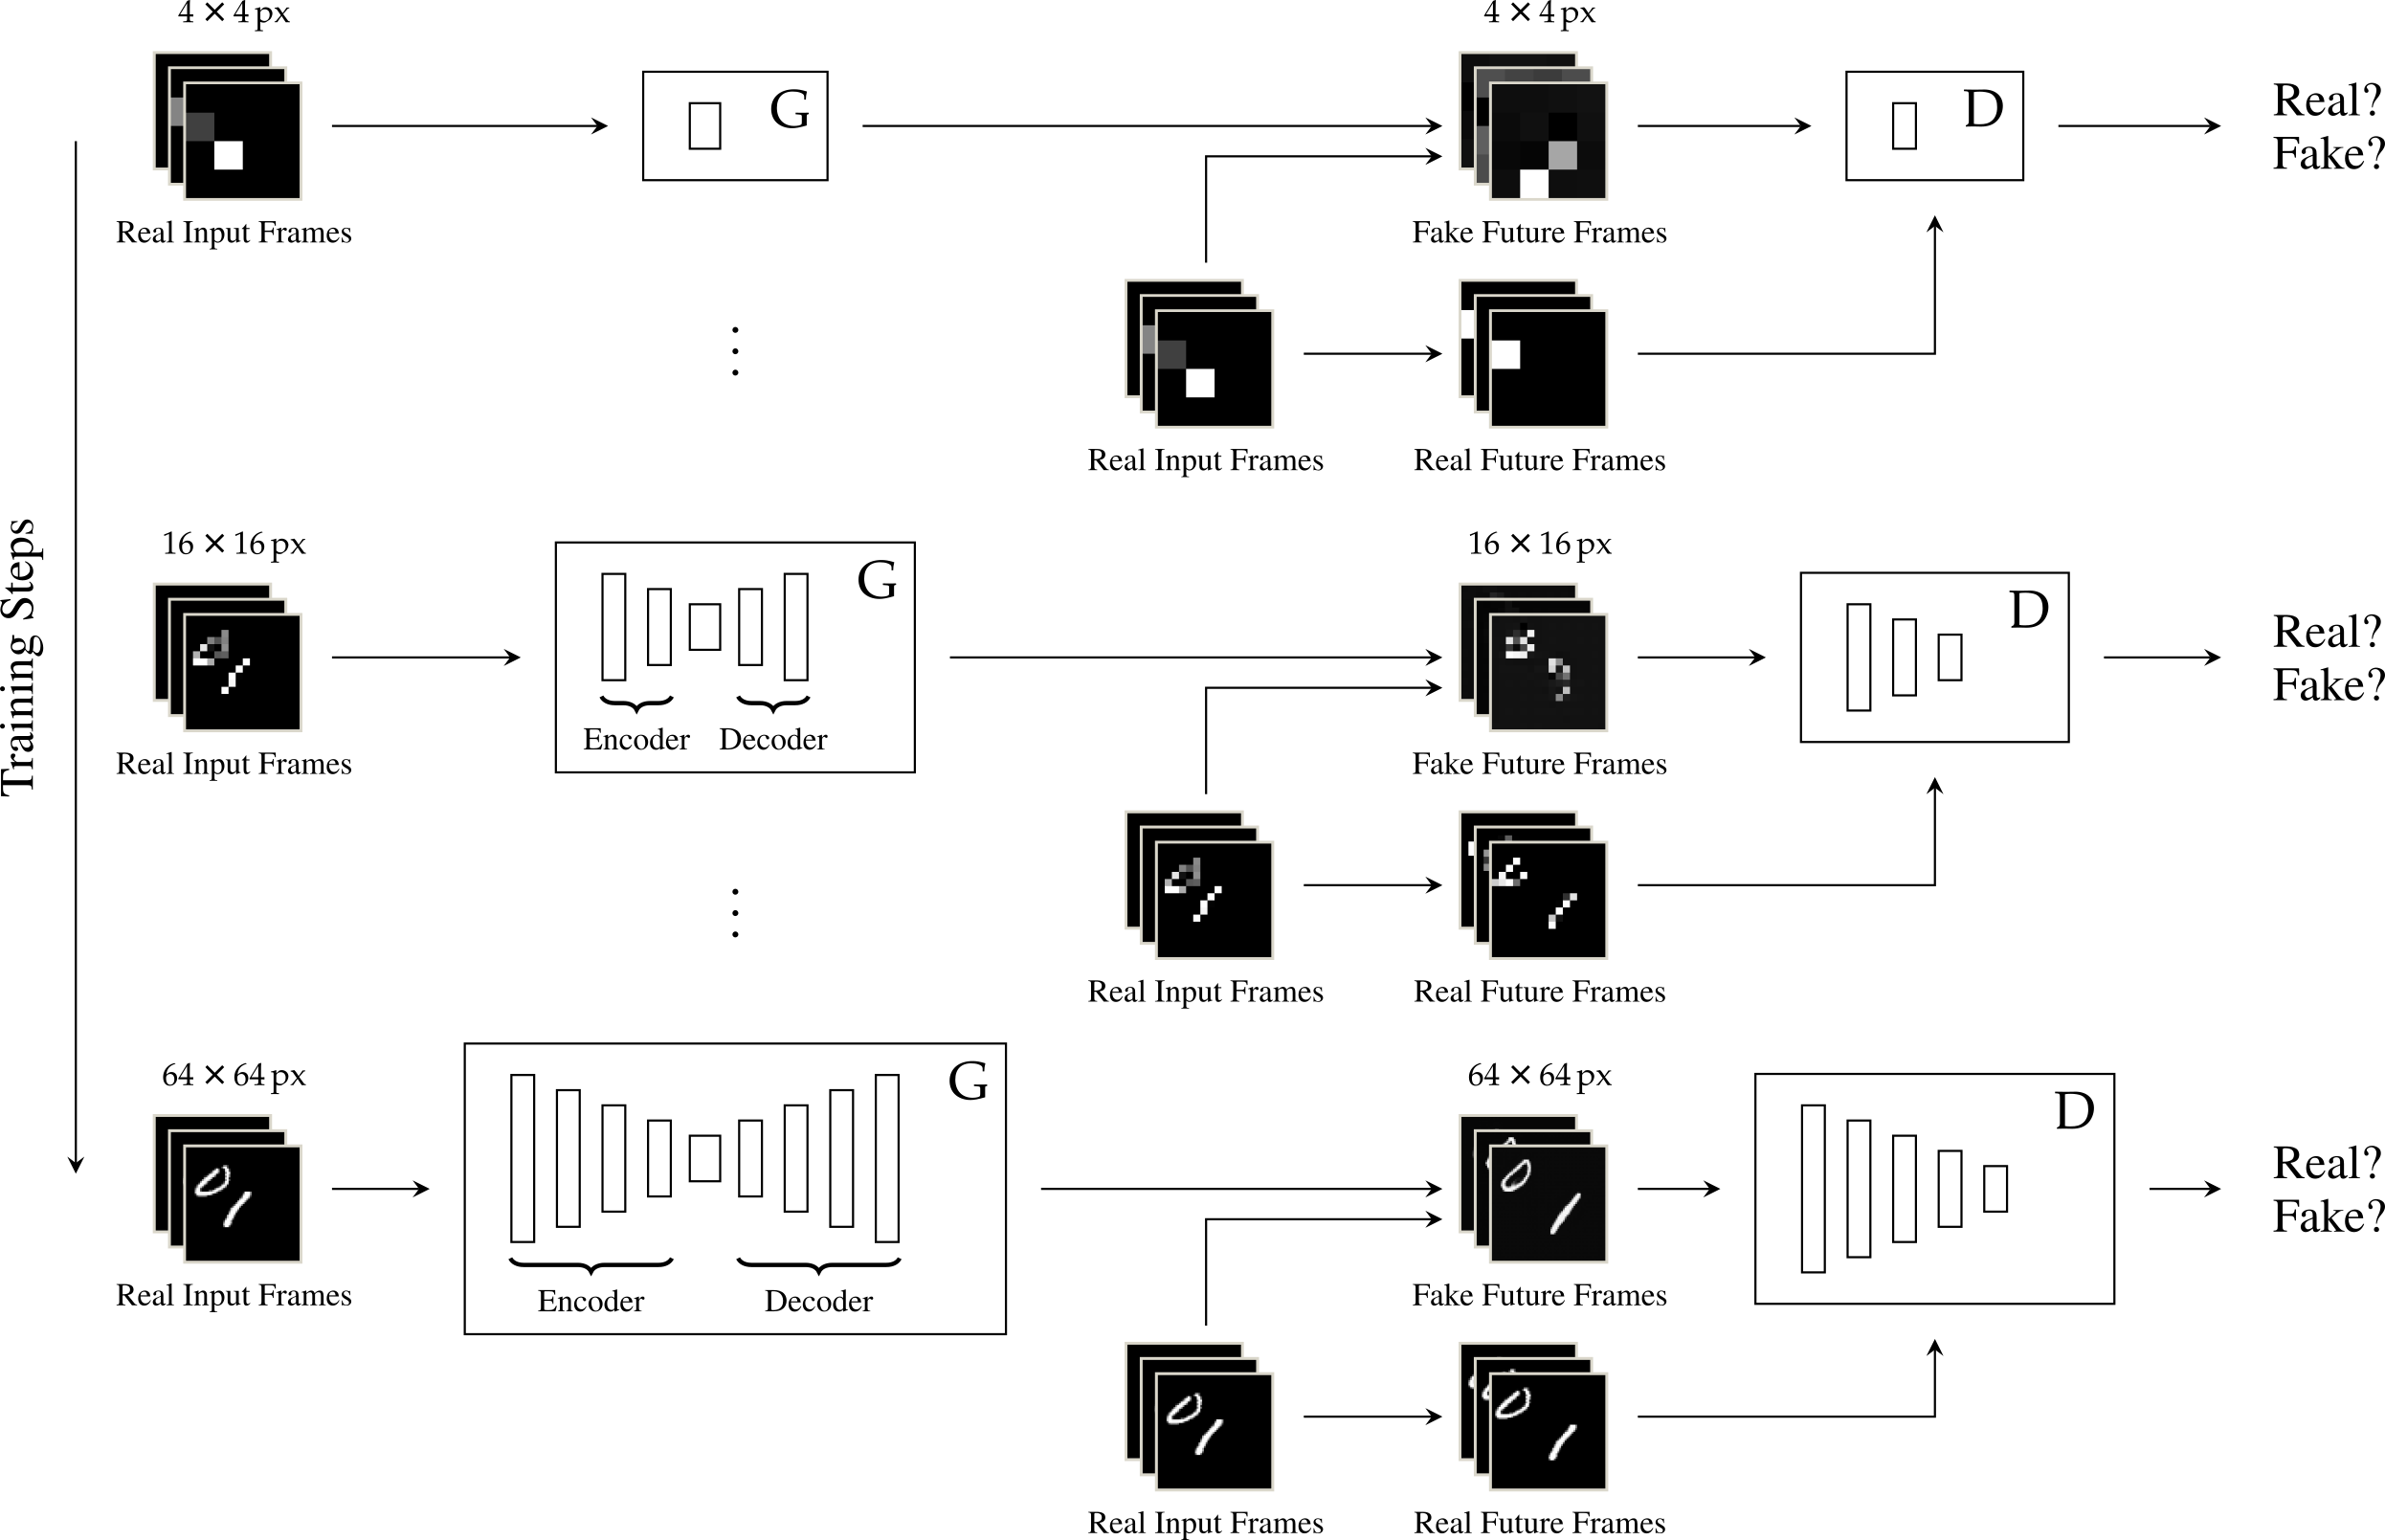
\includegraphics[width=1\textwidth]{figures/futuregan_arch.png}
	\end{center}
	\caption{FutureGAN Architecture}
	\label{fig:futuregan_arch}
\end{figure}

\subsection{SAVP}
\label{subsec:savp}

\newpage
\section{Datasets}
\label{sec:datasets}

\subsection{MovingMNIST}
\label{subsec:mmnist}

\subsection{KTH}
\label{subsec:kth}

\subsection{BAIR}
\label{subsec:bair}

\newpage
\section{Experiments}
\label{sec:experiments}

% \begin{table}
% 	\caption{Summary of Main ConvLSTM Results}
% 	\label{tab:results_summary}
% 	\begin{center}
% 		\begin{tabular}{ l l l l }
% 			\textbf{Dataset} & \textbf{Number of layers} & \textbf{Number of Parameters} & \textbf{Test MSE Loss} \\
% 			MovingMNIST & \\
% 			KTH & \\
% 			BAIR
% 		\end{tabular}
% 	\end{center}
% \end{table}


The main experimental procedure carried out in this report is the training and
testing of the re-implemented Convolutional LSTM model on the MovingMNIST, KTH,
and BAIR datasets, however, in order to more gain a more robust understanding
of LSTM features and limitations, as well as to debug the training mechanisms
in a much simpler setting, it was useful to first test a Linear LSTM model on
one-dimensional sequential data before moving fully to video prediction.

This Linear LSTM was implemented with nearly the same exact architecture as the
Convolutional LSTM, however with Linear layers in place of convolutions, and as
a result, a 2D convolution layer as the final step as opposed to 3D.

% Insert Linear LSTM specifics

\subsection{Sequence Prediction}
\label{subsec:experiment_sp}

Two generated datasets of one-dimensional sequences were implemented, one which
was composed of sin waves with random frequency and phase offset, and another
which represented random points chosen at several steps within the sequence and
simply interpolated using a sinusoidal interpolation function. Both datasets
were normalized to the range $(0, 1)$, with 20 total data points for each
seqeuence. The model was then given the first 10 points and tasked to predict
the last 10.

\subsubsection{Generated Sinusoids}
\label{subsubsec:generated_sins}

Figure \ref{fig:gen_sin_training} shows the model's inferences on a held-out
set of the generated sinusoidal data as the model trains over one epoch. 

\subsection{Video Prediction}
\label{subsec:experiment_vp}

\begin{figure}[H]
	\begin{center}
		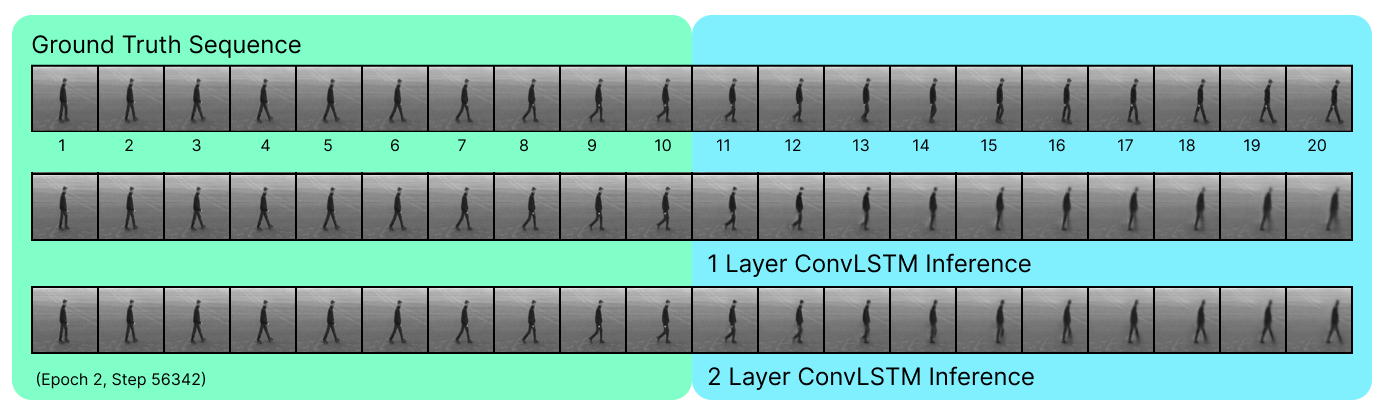
\includegraphics[width=1\textwidth]{images/kth/KTHEpoch2Step56342.png}
	\end{center}
	\caption{Convolutional LSTM Inference on KTH dataset}
	\label{img:lstm_kth_inference}
\end{figure}

\newpage
\section{Conclusion}
\label{sec:conclusion}

% ------------------------------------------------------------------------------
% References 
% ------------------------------------------------------------------------------

\newpage
\bibliography{main}
\newpage

\end{document}

